\documentclass[a4paper, 12pt]{article}

% Essential Packages
\usepackage{amsmath}
\usepackage{amssymb}
\usepackage[top=25mm, bottom=25mm, left=25mm, right=25mm]{geometry}
\usepackage{pgfplots}
\usepackage[inline]{enumitem}
\usepackage{mathtools}
\usepackage{tikz}
\usepackage{fancyhdr}
\usepackage{setspace}
\usepackage{hyperref}

% Misc
\pgfplotsset{compat=1.18}
\usepgfplotslibrary{polar}
\usepgfplotslibrary{fillbetween}
\setlength{\parskip}{3pt}
\setstretch{1.15}
\renewcommand{\headrulewidth}{0pt}
\renewcommand{\footrulewidth}{0pt}
\fancyhf{}

\begin{document}
\pagestyle{empty}

\begin{center}
\textbf{2012-2013 Fall \\MAT123 Midterm II\\19/12/2012}
\end{center}

\begin{enumerate}[leftmargin=*,label=\textbf{\arabic*.}]

\item A 10 m long wire is cut into two pieces. One piece is bent into an equilateral triangle and the other piece is bent into a circle. If the sum of the areas enclosed by each part is minimum, what is the length of each piece?



\item Integrate the following functions, and write each step in detail.

\begin{enumerate}[leftmargin=*,label=\textbf{\alph*.}]
\item $\displaystyle\int\frac{dy}{\sqrt{y}\left(1+\sqrt y\right)^2}$
\item $\displaystyle\int_{\pi/6}^{\pi/4}\frac{\cot x}{\ln(\sin x)}\,dx$
\item $\displaystyle\int\frac{x^3-4x-10}{x^2-x-6}\,dx$
\item $\displaystyle \int\tan x \sec^{123}x\,dx$
\item $\displaystyle\int\sqrt{t-t^2}\,dt$
\item $\displaystyle\int\sqrt{1+\sqrt x}\,dx$
\end{enumerate}

\item Integrate the following functions, and write each step in detail.

\begin{enumerate}[leftmargin=*,label=\textbf{\alph*.}]
\item $\displaystyle \int_0^2\frac{dx}{\sqrt{|x-1|}}$
\item $\displaystyle\int_{-\infty}^{\infty}x^2 e^{-x^3}\,dx$
\end{enumerate}

\item By using the Washer Method, find the volume of the solid generated by revolving the region bounded by the curves $x=y^3$ and $y+x^2=0$ about the $x$-axis.
\end{enumerate}

\newpage
\pagestyle{fancy}
\renewcommand{\headrulewidth}{1pt}
\fancyhead[R]{\textit{2012-2013 Fall Midterm II}}
\fancyhead[L]{\textit{Hacettepe MAT123 Exam Solutions Version 2}}

% Last update: 07/09/2026 01:49

\begin{enumerate}[leftmargin=*,label=\textbf{\arabic*.}]

\item Let $x$ be the length of the wire that is used to form the equilateral triangle. So, $10-x$ is the length of the other piece. The area of the triangle is
\[A_1 = \frac{x^2\sqrt3}{4}\]

The perimeter of the circle is $10-x$. Therefore, $2\pi r = 10-x$, where $r$ is the radius of the circle. The area of the circle can be extracted from the formula $A_2=\pi r^2$. Solve the former equation for $r$, and express the area in terms of $x$.
\[r=\frac{10-x}{2\pi}\,\rightarrow\, A_2 = \pi\left(\frac{10-x}{2\pi}\right)^2 =\frac{100-20x+x^2}{4\pi}\]

Let $A(x)$ be the function of length representing the sum of the areas.
\[A(x) = \frac{x^2\sqrt3}{4}+\frac{100-20x+x^2}{4\pi}\]

Minimize $A(x)$ by taking the first derivative and setting it to $0$.
\[A'(x)=\frac{x\sqrt3}{2} + \frac{x-10}{2\pi}=0\,\rightarrow\,10=x+x\cdot\pi\sqrt3\,\rightarrow\,x=\frac{10}{1+\pi\sqrt3}\]

The length of the piece used to form the triangle is $\displaystyle\frac{10}{1+\pi\sqrt3}$, the length of the other piece is $\displaystyle\frac{10\pi\sqrt3}{1+\pi\sqrt3}$.

\item Integrate the following functions, and write each step in detail.

\begin{enumerate}[leftmargin=*,label=\textbf{\alph*.}]
\item Let $u=1+\sqrt y$, then $\displaystyle du=\frac{dy}{2\sqrt y}$.

\[\int\frac{dy}{\sqrt{y}\left(1+\sqrt y\right)^2}=\int\frac{1}{u^2}\cdot2\,du=-\frac{2}{u}+c=\boxed{-\frac{2}{1+\sqrt y}+C,\quad C\in\mathbb{R}}\]

\item Let $u=\ln(\sin x)$, then $\displaystyle du=\frac{1}{\sin x}\cdot \cos x\,dx$.
\begin{align*}
\int_{\pi/6}^{\pi/4}\frac{\cot x}{\ln(\sin x)}\,dx&=\int\frac1u\,du=\ln|u| + c=\Big[\ln\left|\ln(\sin x)\right| \Big]_{\pi/6}^{\pi/4}\\[1em]&=\ln\left|\ln\frac{\sqrt2}2\right|-\ln\left|\ln\frac12\right|=\ln\frac{\left|\ln\frac{\sqrt2}{2}\right|}{\left|\ln\frac12\right|}\\[1em]&=\ln\left(\frac{\ln2-\ln\sqrt2}{\ln2-\ln1}\right)=\ln\frac12=\boxed{-\ln2}
\end{align*}

\item Attempt a long polynomial division and split into two integrals.
\begin{align*}
I=\int\frac{x^3-4x-10}{x^2-x-6}\,dx&=\int(x+1)\,dx+\int\frac{3x-4}{(x-3)(x+2)}\,dx\\[1em]&=\frac{x^2}2+x+\int\left({\frac{A}{x-3}+\frac{B}{x+2}}\right)\,dx
\end{align*}

Expand the numerators.
\begin{align*}
A(x+2)+B(x-3)&=3x-4\\
x(A+B)+2A-3B&=3x-4
\end{align*}

Solve for $A$ and $B$.
\[
\left.
\begin{array}{ll}
A+B=3\\
2A-3B=-4
\end{array}
\right\}
\quad A=1,\quad B=2
\]

The result is then
\begin{align*}
I &= \frac{x^2}{2}+x+\int\left(\frac{1}{x-3}+\frac{2}{x+2}\right)\,dx \\
  &= \boxed{\frac{x^2}{2}+x+\ln|x-3|+2\ln|x+2|+C,\quad C\in\mathbb{R}}.
\end{align*}

\item Let $u=\sec x$, then $du=\tan x \sec x \,dx$.
\[\int\tan x\sec^{123}x\,dx=\int u^{122}\,du=\frac{u^{123}}{123}+c = \boxed{\frac{\sec^{123}x}{123}+C,\,C\in\mathbb{R}}\]

\item Let $t=\sin^2x$, then $dt=2\sin x\cos x\,dx$.
\begin{align*}\int\sqrt{t-t^2}\,dt&=\int\sqrt{\sin^2x-\sin^4x}\cdot2\sin x \cos x \,dx\\[1em]&=\int\sqrt{\sin^2x\cdot(1-\sin^2x)}\cdot\sin(2x)\,dx\\[1em]&=\int\sin x \cos x\cdot\sin(2x)\,dx\\[1em]&=\frac12\int\sin^2(2x)\,dx=\frac12\int\left(1-\cos^2(2x)\right)\,dx\\[1em]&=\frac12\int\frac{1-\cos(4x)}2\,dx=\frac14\left[x-\frac14\sin(4x)\right]+C,\quad C\in\mathbb{R}\end{align*}

We will try to rewrite the result in terms of $t$.
\[t-t^2 \geq 0\implies 0\leq t \leq 1\]
\[t=\sin^2x \implies\sqrt t = \sin x\implies\arcsin\left(\sqrt t\right) = x\]
\[t=\sin^2x=1-\cos^2x\implies \cos x= \sqrt{1-t}\]
\[\sin(4x)=2\sin(2x)\cos(2x)=4\sin x\cos x\left(2\cos^2x-1\right)=4\sqrt t\cdot\sqrt{1-t}\cdot(1-2t)\]

\vspace{-2em}
\begin{align*}
\int\sqrt{t-t^2}\,dt=\boxed{\frac14\left[\arcsin\left(\sqrt t\right)-\sqrt{t(1-t)}\cdot(1-2t)\right]+c,\,c\in\mathbb{R}}
\end{align*}

\item Let $u=\sqrt{1+\sqrt x}$.
\[u^2 = 1+\sqrt x\implies u^2-1 = \sqrt x\implies\left(u^2-1\right)^2 = x\implies2\left(u^2-1\right)\cdot 2u\,du = dx\]

\vspace{-2em}
\begin{align*}
\int \sqrt{1+\sqrt{x}}\,dx&=\int u \cdot(2u^2-2)\cdot 2u\,du=\int\left(4u^4-4u^2\right)\,du=\frac{4u^5}5-\frac{4u^3}{3} + c\\[1em]&=\boxed{\frac{4\left(\sqrt{1+\sqrt x}\right)^5}5-\frac{4\left(\sqrt{1+\sqrt x}\right)^3}3+c,\,c\in\mathbb{R}}\end{align*}
\end{enumerate}

\item \begin{enumerate}[leftmargin=*,label=\textbf{\alph*.}]
\item\leavevmode

\vspace{-4em}
\begin{align*}
\int_0^2\frac{dx}{\sqrt{|x-1|}}&=\int_0^1\frac{dx}{\sqrt{1-x}} + \int_1^2\frac{dx}{\sqrt{x-1}}=\lim_{S\to1^-}\int_0^S\frac{dx}{\sqrt{1-x}}+\lim_{P\to1^+}\int_P^2\frac{dx}{\sqrt{x-1}}\\[1em]&=\lim_{S\to1^-}\left[-2\sqrt{1-x}\right]_0^S+\lim_{P\to1^+}\left[2\sqrt{x-1}\right]_P^2\\[1em]&=\lim_{S\to1^-}\left[-2\sqrt{1-S}\right]+2\sqrt{1-0}+2\sqrt{2-1}-\lim_{P\to1^+}\left[2\sqrt{P-1}\right]=\boxed4
\end{align*}

\item\leavevmode

\vspace{-4em}
\begin{align*}\int_{-\infty}^{\infty} x^2 e^{-x^{3}}\,dx=\lim_{a\to\infty}\int_{-a}^{a} x^2 e^{-x^{3}}\,dx=\lim_{a\to\infty}-\frac13\left[ e^{-x^3}\right]_{-a}^a=\boxed\infty\end{align*}
\end{enumerate}

\item\leavevmode

\vspace{-2em}
\begin{minipage}{0.45\textwidth}
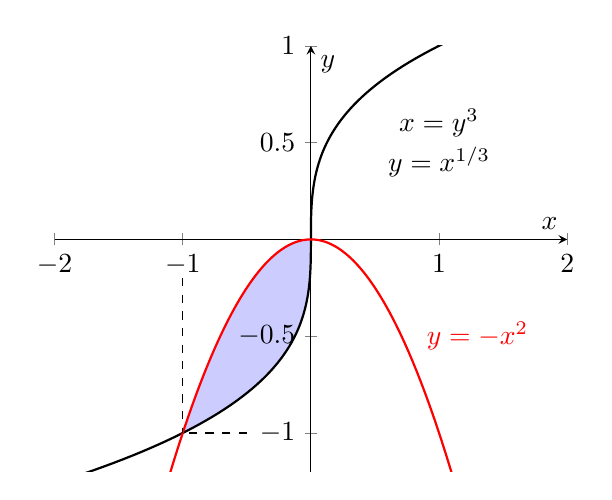
\begin{tikzpicture}
  \begin{axis}[
    axis lines = middle,
    xlabel = {$x$},
    ylabel = {$y$},
    ymin = -1.2, ymax = 1,
    xmin = -2, xmax = 2,
    samples = 200,
    domain = -2:2,
    clip=true,
    scale=0.95,
  ]

  \addplot [
    name path=A,
    domain=-1:0,
    draw=none,
  ] {-x^2};

  \addplot [
    name path=B,
    domain=-1:0,
    draw=none,
  ] ({x^3}, x);

  \addplot [
    fill=blue!20,
  ] fill between[of=A and B];

  \addplot [
    domain=-2:2,
    samples=200,
    thick,
    black,
  ] ({x^3}, x);

  \addplot [
    domain=-2:2,
    samples=200,
    thick,
    red,
  ] {-x^2};

  \draw[dashed] (axis cs:-1,-0.2) -- (axis cs:-1,-1);
  \draw[dashed] (axis cs:-0.5,-1) -- (axis cs:-1,-1);

  \node[red] at (axis cs: 1.3,-0.5) {$y=-x^2$};
  \node at (axis cs: 1,0.6) {$x=y^3$};
  \node at (axis cs: 1,0.4) {$y=x^{1/3}$};

  \end{axis}
\end{tikzpicture}
\end{minipage}
\begin{minipage}{0.5\textwidth}
\begin{align*}
V&=\int_{-1}^0\pi\left[\left(x^{1/3}\right)^2-\left(-x^2\right)^2\right]\,dx\\[1em]&=\pi\int_{-1}^0\left(x^{2/3}-x^4\right)\,dx\\[1em]&=\pi\left[\frac35x^{5/3}-\frac{x^5}{5}\right]_{-1}^0\\[1em]&=\pi\cdot\left[0-\left(-\frac35+\frac15\right)\right]=\boxed{\frac{2\pi}5}
\end{align*}\
\end{minipage}
\end{enumerate}
\end{document}